\documentclass{report}

\usepackage{graphicx}
\usepackage{algorithm}
\usepackage{array}
\usepackage{dsfont}
\usepackage{algpseudocode}
\usepackage{listings}
\usepackage{amsmath}
\usepackage{tikz}
\usepackage{pdfpages}
\usepackage{float}


\usetikzlibrary{trees}
\usetikzlibrary{automata, positioning, arrows}
\DeclareMathOperator{\rank}{rank}
\makeatletter
\newenvironment{sqcases}{%
  \matrix@check\sqcases\env@sqcases
}{%
  \endarray\right.%
}
\def\env@sqcases{%
  \let\@ifnextchar\new@ifnextchar
  \left\lbrack
  \def\arraystretch{1.2}%
  \array{@{}l@{\quad}l@{}}%
}
\makeatother

\usetikzlibrary{calc}


\input{/mnt/fa80f336-3342-4d78-8bfd-a43e434a2cda/Latex/preamble.tex}
\input{/mnt/fa80f336-3342-4d78-8bfd-a43e434a2cda/Latex/macros.tex}
\input{/mnt/fa80f336-3342-4d78-8bfd-a43e434a2cda/Latex/letterfonts.tex}

\title{\Huge{FU08 \-- Automata and Languages}\\Exercise 9}
\author{\huge{NGUYEN Tuan Dung}\\\huge{s1312004}}
\date{January 23, 2025}

\begin{document}

\maketitle

% Cau 1
\qs{Answer the following questions}{
For the grammar: \newline
\begin{equation*}
    \begin{aligned}
    &\mathrm{S} \longrightarrow \mathrm{A1B} \\
    &\mathrm{A} \longrightarrow \mathrm{0A~|~} \lambda \\
    &\mathrm{B} \longrightarrow \mathrm{0B~|~1B~|~}\lambda \\
    \end{aligned}
\end{equation*}
\newline
And the strings 00101 and 1001, give:\newline
\\
 a. The leftmost derivation\newline
 b. The rightmost derivation\newline
 c. The parse tree}

\sol{\newline
\begin{minipage}[t]{0.48\textwidth}
    a. \textbf{For the string 00101:}\newline
    $ S \rightarrow
    A1B \rightarrow
     0A1B \rightarrow
      00A1B \rightarrow
       001B \rightarrow
        0010B \rightarrow
         00101B \rightarrow
          00101\lambda $
    \newline
    We have sucessfully derived the input string 00101.
\end{minipage}
\hfill
\begin{minipage}[t]{0.48\textwidth}
    \textbf{For the string 1001:}\newline
    $ S \rightarrow
     A1B \rightarrow
     1B \rightarrow
      10B \rightarrow
      100B \rightarrow
      1001B \rightarrow
      1001 \lambda $
    \newline
    We have sucessfully derived the input string 1001.
\end{minipage}
\newline
\noindent \newline
\begin{minipage}[t]{0.48\textwidth}
    b. \textbf{For the string 00101:}\newline
    $ S \rightarrow
    A1B \rightarrow
    A10B \rightarrow
    A101B \rightarrow
    A101 \rightarrow
    0A101 \rightarrow
    00A101 \rightarrow
    00 \lambda 101 $
    \newline
    We have sucessfully derived the input string 00101.
\end{minipage}
\hfill
\begin{minipage}[t]{0.48\textwidth}
    \textbf{For the string 1001:}\newline
    $ S \rightarrow
    A1B \rightarrow
    A10B \rightarrow
    A100B \rightarrow
    A1001B \rightarrow
    A1001 \rightarrow
    \lambda 1001 $
    \newline
    We have sucessfully derived the input string 1001.
\end{minipage}
\newline
\noindent \newline
\begin{minipage}[t]{0.48\textwidth}
    c. \textbf{For the string 00101:}\newline
    \begin{tikzpicture}
        [
            level 1/.style={sibling distance=15mm},
            level 2/.style={sibling distance=12mm},
            level 3/.style={sibling distance=10mm},
            level 4/.style={sibling distance=7mm},
        ]
        \node {S}
            child { node {A}
                child { node {0} }
                child { node {A}
                    child { node {0} }
                    child { node {A}
                        child { node {$\lambda$} } 
                    } 
                }
            }
            child { node {1} }
            child { node {B} 
                child { node {0} }
                child { node {B}
                    child { node {1} }
                    child { node {B} 
                        child { node {$\lambda$} } 
                    }
                }
            };
    \end{tikzpicture}
\end{minipage}
\hfill
\begin{minipage}[t]{0.48\textwidth}
    \textbf{For the string 1001:}\newline
    \begin{tikzpicture}
        [
            level 1/.style={sibling distance=15mm},
            level 2/.style={sibling distance=15mm},
            level 3/.style={sibling distance=12mm},
            level 4/.style={sibling distance=9mm},
            level 5/.style={sibling distance=6mm},
        ]
        \node {S}
            child { node {A} }
            child { node {1} }
            child { node {B} 
                child { node {0} }
                child { node {B}
                    child { node {0} }
                    child { node {B} 
                        child { node {1} }
                        child { node {B}
                            child { node {$\lambda$} }
                        } 
                    }
                }
            };        
    \end{tikzpicture}
\end{minipage}
}

\pagebreak

% Cau 2
\qs{Show that the following grammar is ambiguous}{
    \begin{equation*}
        \begin{aligned}
            & \mathrm{S} \longrightarrow \mathrm{AB~|~aaB} \\
            & \mathrm{A} \longrightarrow \mathrm{a~|~Aa} \\
            & \mathrm{B} \longrightarrow \mathrm{b}
        \end{aligned}
    \end{equation*}
}

\sol{\newline
Take a random input string w = aab. Let us construct the parsing tree of the grammar and see if the derivation tree is unique.

\begin{minipage}[t]{0.48\textwidth}
\noindent \textbf{For the string aab:}\newline
\begin{tikzpicture}
    [
        level 1/.style={sibling distance=15mm},
        level 2/.style={sibling distance=15mm},
        level 3/.style={sibling distance=12mm},
        level 4/.style={sibling distance=9mm},
        level 5/.style={sibling distance=6mm},
    ]
    \node {S}
        child { node {aa} }
        child { node {B} 
            child { node {b} } 
            };        
\end{tikzpicture}
\end{minipage}
\hfill
\begin{minipage}[t]{0.48\textwidth}
    \noindent \textbf{For the string aab:}\newline
    \begin{tikzpicture}
        [
            level 1/.style={sibling distance=15mm},
            level 2/.style={sibling distance=15mm},
            level 3/.style={sibling distance=12mm},
            level 4/.style={sibling distance=9mm},
            level 5/.style={sibling distance=6mm},
        ]
        \node {S}
            child { node {A}
                child { node {A}
                    child { node {a} } 
                }
                child { node {a} } 
            }
            child { node {B} 
                child { node {b} } 
            };    
    \end{tikzpicture}
    \end{minipage}
Acknowledge that the same input string w = aab have two different parsing tree representation. Hence, the grammar is ambiguous.
}
\newline
% Cau 3
\qs{Find s-grammar for the following languages}{
    a. L(r) where r = aaa^*b+b\\
    b. ~L = \{a^nb^n : n \geq 1\}
}

\sol{\newline
\begin{minipage}[t]{0.48\textwidth}
a. \newline
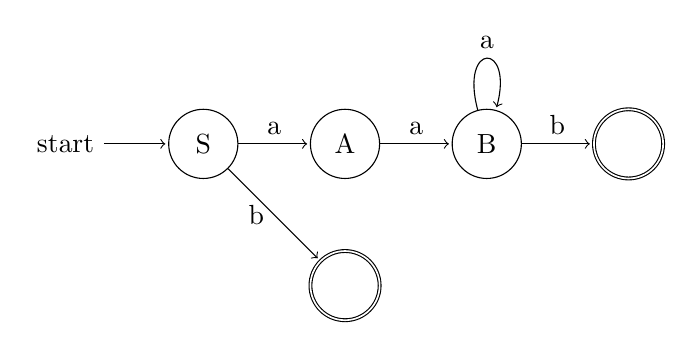
\begin{tikzpicture}[shorten >=1pt, scale=1.8, node distance=1.8cm, on grid, auto][h]
    \node[state, initial] (s) {S};
    \node[state] (a) [right=of s] {A};
    \node[state] (b) [right=of a] {B};
    \node[state, accepting] (c) [right=of b] {};
    \node[state, accepting] (d) [below of=a] {};

    \path[->]  
    (s) edge node {a} (a)
        (s) edge node[left] {b} (d)
    (a) edge node {a} (b)
    (b) edge[loop above] node {a} (b)
        (b) edge node {b} (c);
\end{tikzpicture}
\end{minipage}
\hfill
\begin{minipage}[t]{0.48\textwidth}
    ~\newline
From the automaton, we construct our simple grammar.
\begin{equation*}
    \begin{aligned}
        & S \longrightarrow \mathrm{aA~|~b} \\
        & A \longrightarrow \mathrm{aB} \\
        & B \longrightarrow \mathrm{aB~|~b}
    \end{aligned}
\end{equation*}
\end{minipage}
\\~\\
\begin{minipage}[t]{0.48\textwidth}
    b. \newline
    Construct a simple grammar for L($aa^*bb^*$). \newline
    \begin{tikzpicture}[shorten >=1pt, scale=1.8, node distance=1.8cm, on grid, auto][h]
        \node[state, initial] (s) {S};
        \node[state] (a) [right=of s] {A};
        \node[state, accepting] (c) [right=of a] {B};
    
        \path[->]  
        (s) edge node {a} (a)
        (a) edge[loop above] node {a} (a)
            (a) edge node {b} (b)
        (b) edge[loop above] node {b} (b);
    \end{tikzpicture}
\end{minipage}
\hfill
\begin{minipage}[t]{0.48\textwidth}
    ~\newline
    From the automaton, we construct our simple grammar.
    \begin{equation*}
        \begin{aligned}
            & S \longrightarrow \mathrm{aA} \\
            & A \longrightarrow \mathrm{aAB~|~b} \\
            & B \longrightarrow \mathrm{b}
        \end{aligned}
    \end{equation*}
    \end{minipage}

}
\end{document}
